% V5 Türkçe çalışma çevirisi. Dergiye gönderilecek metin main.tex'tir.
% Tablolar: ../analysis/build_tables.py, ardından ../analysis/build_tr.py.
\documentclass[journal]{IEEEtran}
\usepackage[T1]{fontenc}
\usepackage[utf8]{inputenc}
\usepackage[turkish,shorthands=off]{babel}
\usepackage{amsmath,amssymb,amsfonts}
\usepackage{graphicx,booktabs}
\usepackage{adjustbox}
\usepackage{url}
\usepackage[hidelinks]{hyperref}

\newtheorem{proposition}{Önerme}
\newtheorem{theorem}{Teorem}
\newtheorem{corollary}{Sonuç}
\newtheorem{definition}{Tanım}
\addto\captionsturkish{\renewcommand{\IEEEkeywordsname}{Anahtar Kelimeler}}
\renewcommand{\IEEEproofname}{İspat}

\newcommand{\method}{Fed-MDBSCAN-G}
\newcommand{\rd}{\mathrm{rd}}
\newcommand{\BER}{\mathrm{BER}}
\newcommand{\BUC}{\mathrm{BUC}}

\begin{document}

\title{Heterojen Federe Öğrenmede Dürüst İstemci\\Dışlama ve Uzlaşma Testinin Sınırları}

\author{Sebahattin~Gökçen~Özden ve Kadir~Sarıkaya%
\thanks{Bu belge, İngilizce gönderim sürümünün yazarlar için hazırlanmış Türkçe çalışma çevirisidir; dergiye gönderilecek metin İngilizce sürümdür. Sayılar İngilizce sürümle birebir karşılaştırılabilsin diye ondalık ayırıcı olarak nokta kullanılmıştır.}%
\thanks{S. G. Özden, Bilgisayar Mühendisliği Bölümü, Mühendislik ve Mimarlık Fakültesi, Tokat Gaziosmanpaşa Üniversitesi, Tokat, Türkiye (e-posta: sebahattin.ozden0025@gop.edu.tr; ORCID: \mbox{0009-0008-9280-444X}).}%
\thanks{K. Sarıkaya, Endüstri Mühendisliği Bölümü, Mühendislik ve Mimarlık Fakültesi, Tokat Gaziosmanpaşa Üniversitesi, Tokat, Türkiye (ORCID: \mbox{0000-0001-9015-6209}).}%
\thanks{Sorumlu yazar: Sebahattin Gökçen Özden.}}

\markboth{IEEE TRANSACTIONS ON INFORMATION FORENSICS AND SECURITY için makale (Türkçe çalışma çevirisi)}{Özden ve Sarıkaya: Dürüst İstemci Dışlama ve Uzlaşma Testinin Sınırları}
\maketitle

\begin{abstract}
Sunucu tarafı federe öğrenme savunmaları, zehirleme saldırılarını hafifletmek için istemci güncellemelerini filtreler. Veri dağılımları yüksek derecede heterojen (IID olmayan) olduğunda istatistiksel olarak sıra dışı dürüst güncellemeler çoğu zaman aykırı görünür. Oysa önceki değerlendirmeler ağırlıklı olarak saldırılı turlardaki başarımı raporlar ve dürüst istemcileri yanlışlıkla reddetmenin kritik bedeli ölçülmeden kalır. Bu boşluğu kapatmak için, aralarında geometrik medyan kabul bölgesine dayanan özgün çok yoğunluklu kümeleme filtremiz Fed-MDBSCAN-G'nin de bulunduğu sekiz birleştirme kuralını dört veri kümesinde, üç heterojenlik düzeyinde (Dirichlet $\alpha \in \{0.5, 0.1, 0.01\}$) ve beş saldırı ailesinde sistematik olarak değerlendiriyoruz. Kapsamlı saldırgansız değerlendirmelerimiz ciddi bir dürüst istemci dışlama sorununu ortaya koyar: Multi-Krum ve FLAME gibi referans yöntemler dürüst gönderimlerin sırasıyla \%32.2'sine ve \%48.9'una kadarını dışlar; heterojen dürüst gruplar için tasarlanan Fed-MDBSCAN-G bile güçlü heterojenlik altında benzer bir payı dışlar; son doğruluk ise düz ortalamanın 65.55 yüzde puana kadar altına düşer. Uzaklık kısıtlı saldırılar altında Multi-Krum ve FLAME, koşulların çoğunda yalnızca dürüst istemcileri reddederek başarısız olur. Ayrıca Fed-MDBSCAN-G'nin küme doğrulama aşamasının ilk kabul edilen güncellemelerden oluşan hiçbir grubu reddedemeyeceği bir yeter koşul türetiyoruz; bu koşul beş adımlı koşumların saldırılı kontrol noktalarının neredeyse tamamında, kanonik olanların ise üçte birinden azında sağlanır. Kopyalanmış saldırganların bu kümeleme aşamalarını uzaklık manipülasyonuyla değil aşırı yoğun kümelenme yoluyla atlattığını ve sonraki filtreleme aşamaları kaldırıldığında ortalama son doğruluğun neredeyse hiç değişmediğini gösteriyoruz. Bu bulgular, değerlendirilen kümeleme tabanlı ve geometrik uygulamaların yüksek heterojenlik altındaki sistemik başarısızlıklarını aydınlatır. Bu nedenle gelecekteki savunma değerlendirmelerinin, saldırgansız koşullardaki dürüst istemci dışlama oranlarını ve doğruluk kaybını saldırı tespiti ve saldırı başarısı ölçütleriyle birlikte raporlamasını savunuyoruz.
\end{abstract}

\begin{IEEEkeywords}
Federe öğrenme, zehirleme, dayanıklı birleştirme, veri heterojenliği, yanlış pozitifler, kümeleme tabanlı savunmalar.
\end{IEEEkeywords}
\IEEEpeerreviewmaketitle

\section{Giriş}
\IEEEPARstart{F}{edere} öğrenme (federated learning, FL), hassas yerel verileri merkezde toplamadan dağıtık istemciler arasında ortak model eğitimini mümkün kılar~\cite{mcmahan2017}. Bu yaklaşım, verinin doğası gereği heterojen ve bağımsız özdeş dağılımlı olmadığı (IID olmayan, non-IID) Nesnelerin İnterneti (Internet of Things, IoT) ve cihazlar arası (cross-device) uygulamalar için özellikle dönüştürücüdür. Ne var ki bu merkeziyetsizlik önemli açıklar doğurur: kötü niyetli istemciler global modeli bozmak için zehirlenmiş güncellemeler (poisoned updates) gönderebilir ya da manipüle edilmiş verilerle eğitim yapabilir~\cite{fang2020,bagdasaryan2020,xie2020dba}. Buna karşılık dayanıklı birleştirme (robust aggregation) algoritmalarını, yoğunluk tabanlı filtrelemeyi (density-based filtering) ve güven önyüklemesini (trust bootstrapping) kapsayan zengin bir sunucu tarafı savunma literatürü oluşmuştur~\cite{blanchard2017,nguyen2022flame,cao2021fltrust,miao2022privacy}.

Bir filtreleme savunmasının tasarımı temelde ikili bir göreve dayanır: kötü niyetli saldırganları güvenilir biçimde dışlarken dürüst istemcilerin yararlı katkılarını (honest contributions) korumalıdır. Uygulamada istatistiksel heterojenlik bu ikili görevi son derece zorlaştırır. Nadir sınıflara ya da alışılmadık yerel veri dağılımlarına sahip dürüst istemciler, turun merkezî eğiliminden belirgin biçimde sapan ve bu yüzden aykırı görünen güncellemeler üretebilir. Buna karşılık gelişmiş, koordineli saldırılar dürüst dağılıma yakın duracak biçimde tasarlanabilir~\cite{baruch2019,shejwalkar2021}. Önceki çalışmalar veri heterojenliğinin dayanıklı birleştirmeyi zayıflatabileceğini ya da yakınsamayı bozabileceğini kabul etmiştir~\cite{liu2023byzantine,li2025heterogeneity,ye2025illusion,bellachia2026sok}; Li vd. ise bazı birleştirme şemalarının hiç Bizans istemcisi yokken bile başarısız olduğunu gözlemlemiştir~\cite{li2024experimental}. Ne var ki bu değerlendirmeler doğruluğu ya da saldırılı turlardaki tespiti raporlar; saldırgansız turlarda dürüst istemcileri yanlışlıkla reddetmenin (yanlış pozitifler, false positives) işletimsel bedeli ve buna yol açan karar aşaması büyük ölçüde ölçülmeden kalır. İstatistiksel olarak sıra dışı dürüst güncellemeleri ayrım gözetmeden atan bir savunma, hiç saldırgan yokken bile model kapsamından, doğruluktan ve adaletten (fairness) ödün verir~\cite{singh2023fair,touat2023bias,ajibuwa2025fairness}.

Bu ödünleşimi incelemenin önemi, standart federe öğrenme kıyaslamalarındaki (benchmark) kritik bir kör noktayı ortaya çıkarmasında yatar: saldırı altında son derece etkili görünen savunmalar, dürüst istemcilere ciddi ve ölçülmemiş fayda kayıpları yükleyebilir. Farklı Dirichlet yoğunlaşma (Dirichlet concentration) değerlerinde saldırgansız (adversary-free) koşullarda değerlendirildiğinde Multi-Krum ve FLAME gibi yerleşik savunmalar dürüst güncellemelerin \%32.2'sine ve \%48.9'una kadarını dışlar ve temiz test doğruluğunu düz ortalamaya göre 65.55 yüzde puana kadar düşürür. Heterojen dürüst grupları tanımak üzere tasarlanmış olmasına karşın kendi bileşik filtremiz \method{} de $\alpha=0.01$ koşulunda dürüst güncellemelerin \%42.6'sına kadarını dışlar. Ayrıca aynı büyüklükte rastgele bir güncelleme altkümesini tutmak gibi basit bir yaklaşımın $\alpha=0.01$ koşulunda Multi-Krum'u 43.7 yüzde puana kadar geride bırakabildiğini buluyoruz; bu da başarımdaki bu çöküşü kohort boyutundaki küçülmenin değil, geometrik seçim ölçütlerinin kendisinin doğurduğunu gösterir. Bu bulgular, yalnızca saldırı altında yapılan değerlendirmelerin pratik fayda hakkında eksik ve yanıltıcı olabilecek bir tablo sunduğunu vurgular.

Önceki deneysel çalışmalar~\cite{li2024experimental}, heterojenliği gözeten dayanıklı birleştirme yöntemleri~\cite{liu2023byzantine} ve uyarlanabilir kümeleme savunmalarıyla~\cite{wang2023adaptive} karşılaştırıldığında bu çalışma hem tanısal yöntemiyle hem de kuramsal nitelendirmesiyle ayrışır. Savunmaları kara kutu olarak ele almak yerine çok aşamalı geometrik filtreleme hatlarının (pipeline) mimari bir otopsisini yapıyoruz~\cite{mia2025bart}. Bu analizi, geometrik medyan tabanlı bir sınırlayıcı bölgeyi paylaşılan komşu tabanlı çok yoğunluklu kümelemeyle~\cite{qian2024mdbscan} birleştiren tipik bir örnek (archetype) olan \method{} üzerinde yürütüyoruz. Kayıtlı güncelleme yörüngeleri boyunca tek tek karar aşamalarını yalıtarak bileşik savunmaların \emph{neden} başarısız olduğunu inceliyoruz: dürüst istemci dışlamasından hangi algoritmik aşamanın sorumlu olduğunu belirliyor ve bu başarısızlıkları yöneten matematiksel yeter koşulları (sufficient conditions) türetiyoruz.

Katkılarımız şunlardır:
\begin{itemize}
    \item \textbf{Sistematik saldırgansız değerlendirme:} Sekiz sunucu tarafı kural, dört veri kümesi ve üç Dirichlet yoğunlaşma değeri ($\alpha\in\{0.5,0.1,0.01\}$) üzerinde kapsamlı bir saldırgansız değerlendirme yapıyoruz. Dürüst istemci dışlama oranını (benign exclusion rate, $\BER$) ve son doğruluğu saldırılı ölçütlerden bağımsız olarak ölçerek Multi-Krum ve FLAME~\cite{nguyen2022flame} gibi standart referans yöntemlerin yol açtığı ciddi doğruluk kaybını sistematik olarak nicelleştiriyoruz.
    \item \textbf{Koşullu geometrik ve dışbükeylik analizi:} Çok aşamalı savunmaların karar yollarını (decision path) çözümlemek için küme içerme (set containment) ve dışbükey zarf yarıçap sınırlarına dayanan biçimsel bir kuramsal çerçeve kuruyoruz. Küme merkezi doğrulamasının (centroid validation) aday grupları reddetmesinin matematiksel olarak olanaksız olduğu yeter koşulları kanıtlıyoruz; bu koşullar beş adımlı koşumların 36 saldırılı kontrol noktasının 35'inde, kanonik koşumlarınkinin ise yalnızca 72'de 22'sinde sağlanır ve sağlandıkları yerde ikincil kümeleme aşamalarının dürüst kabul sınırı içindeki aykırı değerleri neden ayıklayamadığını açıklar.
    \item \textbf{Karar yolu yörünge tanılaması:} Kayıtlı eğitim kontrol noktalarında (checkpoint) sabit matris yeniden oynatmalarıyla (replay) yönlendirme mekanizmalarını doğrulama kurallarından ayırıyoruz. Kopyalanmış saldırganların çok yoğunluklu kümelemeden uzaklık manipülasyonuyla değil aşırı yoğunluk birikimiyle kaçtığını ve böylece sonraki aşamaları etkisiz bıraktığını gösteriyor, gelecekteki değerlendirmelerde dürüst istemci dışlama ölçütlerinin zorunlu tutulması için somut öneriler sunuyoruz.
\end{itemize}

Makalenin geri kalanı şöyle düzenlenmiştir. Bölüm~\ref{sec:related}--\ref{sec:protocol} ilgili çalışmaları, sistem modelini, koşullu analizi ve deney protokolümüzü; Bölüm~\ref{sec:benign}--\ref{sec:conclusion} ise deneysel bulgularımızı ve bunların sonuçlarını ele alır.

\section{İlgili Çalışmalar}\label{sec:related}
\subsection{Dayanıklı birleştirme ve güven önyüklemesi}
Geometrik medyan ile birleştirme, koordinat bazında kestiriciler ve komşuluk tabanlı seçim gibi geleneksel dayanıklı birleştirme teknikleri, Bizans (Byzantine) saldırganlarının etkisini çoğunlukla IID varsayımları altında sınırlamak için geliştirilmiştir~\cite{blanchard2017,yin2018,pillutla2022rfa}. Daha yakın zamanda alan, özellikle FLTrust ile tanınan güven önyüklemesi mekanizmalarına yönelmiştir~\cite{cao2021fltrust}; FLTrust, yerel güncellemelere güven puanı atamak için sunucu tarafında tutulan temiz bir kök veri kümesinden (root dataset) yararlanır. Bu yaklaşımın uzantıları, blok zinciri tabanlı ve gizliliği koruyan dayanıklı birleştirmeyi de incelemiştir~\cite{miao2022privacy}. Bu kuramsal sınırlar ve yapılar belirli varsayımlar altında dayanıklı birleştirme sağlasa da~\cite{karimireddy2022bucketing,allouah2023mixing}, kritik bir işletimsel ölçütü, yani yüksek derecede heterojen turlarda dürüst istemcilerin açık kabul ve dışlama oranlarını çoğu zaman göz ardı eder. Temel küme ve dışbükeylik argümanlarımız (Bölüm~\ref{sec:theory}) optimizasyon hatası sınırlarının yerini almak için değil, tam da bu katılım kararlarını çözümlemek için tasarlanmıştır.

\subsection{Kümeleme tabanlı savunmalar ve IID olmayan verinin güçlükleri}
Gelişmiş arka kapı (backdoor) ve zehirleme saldırılarına karşı güncel literatür giderek daha fazla yoğunluk ve kümeleme tabanlı filtrelemeye başvurmaktadır. FLAME~\cite{nguyen2022flame} HDBSCAN kümelemesini kırpma ve diferansiyel gizlilik gürültüsüyle birleştirirken DeepSight model davranışı incelemesini kümelemeyle birlikte kullanır~\cite{rieger2022deepsight}. Yakın tarihli katkılar bu alanı ilerletmiştir: Wang vd., IID olmayan senaryolarda değişen saldırgan oranlarıyla başa çıkmak için uyarlanabilir dayanıklı savunma algoritması RDFL'i önermiş~\cite{wang2023adaptive}, Mia ve Amini ise kurumlar arası (cross-silo) aykırı değer tespiti için çok ölçütlü bir oylama mekanizması olan BART-FL'i geliştirmiştir~\cite{mia2025bart}. Dikkat çeken diğer çok aşamalı çerçeveler arasında CrowdGuard, MESAS, FLShield ve Fedward vardır~\cite{rieger2024crowdguard,krauss2023mesas,kabir2023flshield,chen2023fedward}.

Bu ilerlemelere karşın IID olmayan ortamlarda yoğunluk tabanlı filtreleme sorunlu olmayı sürdürmektedir. Yanlış pozitif oranlarını düşürmek için uyarlanabilir komşuluk seçimleri ve çok ölçütlü yoğunluk kestirimleri önerilmiştir~\cite{ramana2026alldd}; ancak bu değerlendirmeler neredeyse yalnızca saldırgan varken yapılmıştır. Çalışmamız bu değişkeni yalıtır: MDBSCAN'deki~\cite{qian2024mdbscan} göreli yoğunluk bölümlemesini (relative-density partitioning) geometrik bir bileşik yöntem olan Fed-MDBSCAN-G'ye uyarlıyor ve yöntemin yanlış pozitif dışlama oranını tümüyle dürüst, yüksek derecede IID olmayan ortamlarda titizlikle değerlendiriyoruz.

\subsection{Dürüst istemci dışlama, adalet ve değerlendirme yöntemi}
Dayanıklı birleştirmenin yan etkisi, yani istatistiksel olarak sıra dışı ama dürüst istemcilerin dışlanması, federe öğrenmede adalet ve yanlılık üzerine yeni tartışmalar başlatmıştır~\cite{singh2023fair,touat2023bias,ajibuwa2025fairness}. Yakın tarihli deneysel çalışmalar, veri heterojenliğinin savunma başarımını ciddi biçimde kötüleştirdiğini ve çoğu zaman saldırganların yüksek derecede dağınık bir dürüst popülasyonun içinde başarıyla gizlenmesine yol açtığını doğrular~\cite{li2025heterogeneity,ye2025illusion,bellachia2026sok}. Şans köşegeninin (chance diagonal) altına düşen çalışma noktalarına (operating point), örneğin negatif Youden indeksine ilişkin gözlemlerimiz bu yakın tarihli bulgularla uyumludur. Ayrıca savunma değerlendirmelerinin dürüst istemcilere karşı yanlış pozitifleri raporlaması ve dürüst istemci dışlamasını açıkça ölçmesi gerektiği yönünde giderek güçlenen bir görüş birliği vardır~\cite{djemaa2026heterogeneity,abad2025evaluation}. Çalışmamız bu çağrıya doğrudan yanıt verir. Saldırgansız kontroller ve negatif $J$ tek başına yeni değildir~\cite{ye2025illusion,bellachia2026sok,li2024experimental}; bizim katkımız bunları tur başına dışlama sayımlarıyla, ayrıntılı karar yolu takibiyle ve koşullu matematiksel analizle birleştirmektir.

Şans köşegeninin altındaki çalışma noktaları önceki çalışmalarda da görülür. Bellachia vd.'nin Tablo~8'i, IID olmayan bir IBA koşulunda FLAME için $\mathrm{TPR}=0$ ve $\mathrm{FPR}=0.45$ raporlar~\cite{bellachia2026sok}. Ye vd.'nin Tablo~V'inde $\mathrm{Dir}(0.1)$ için verilen TPR/TNR çiftleri, FoolsGold ve CrowdGuard için sırasıyla $J=-4.15$ ve $-6.8$ yüzde puan anlamına gelir~\cite{ye2025illusion}. Dolayısıyla negatif $J$, burada değerlendirilen uzaklık kısıtlı yoklamalara (probes) özgü değildir.

Başka çalışmalardaki oranlar dikkat ister. Ye vd., FLAME için $\mathrm{Dir}(0.5)$ koşulunda \%73.29, $\mathrm{Dir}(0.1)$ koşulunda \%54.87 TNR, yani \%26.71 ve \%45.13 FPR raporlar; ancak bu değerler farklı kohort boyutları ve paydalarla saldırılı turlardan gelir, bu nedenle yapılandırmamızın \%48.89 üst sınırını ne doğrular ne de çürütür.

\section{Sistem Modeli ve Karar Kuralları}\label{sec:model}
\subsection{Protokol ve tehdit modeli}
$r$ turunda $i$ istemcisi $w_r$ modelini alır ve yerel model farkı (local model delta) $u_{r,i}=w^{\mathrm{local}}_{r,i}-w_r$ güncellemesini gönderir. $B_r$ indekslerini kabul eden düz ortalama (uniform mean) filtresi $w_{r+1}=w_r+|B_r|^{-1}\sum_{i\in B_r}u_{r,i}$ güncellemesini uygular. Paneldeki diğer kurallar kendi ağırlıklandırma, kırpma veya koordinat bazında birleştirme yöntemlerini kullanır; düz ve örnek ağırlıklı ortalama (sample-weighted mean) ayrı referans yöntemler olarak yer alır.

Sunucu güvenilirdir ve istemci kimlikleri sabittir. Saldırganlar kendi eğitim verilerini veya gönderdikleri güncellemeleri kontrol eder. Min-Max ve Min-Sum yoklamaları her şeyi bilen (omniscient) türdendir: mevcut dürüst güncellemeleri de gözlemler ve ilgili uzaklık sınırına uyan ortak bir kötü niyetli vektör oluştururlar. Gerçek kötü niyetli kimlikler bu saldırıları oluşturmak ve kararları puanlamak için kullanılır; savunmaya hiçbir zaman girdi olarak verilmez.

$U=\{1,\ldots,n\}$ gönderimleri (submission) indekslesin; $H$ ve $A$ da $U$ kümesini dürüst ve saldırgan katılımcılara ayırsın. $|H|>0$ olsun. Kabul edilen $B$ indeksleri için $\mathrm{FPR}=|H\setminus B|/|H|$ ve $|A|>0$ olduğunda $\mathrm{TPR}=|A\setminus B|/|A|$ tanımlanır. Bunların farkı Youden indeksi (Youden's index) $J=\mathrm{TPR}-\mathrm{FPR}$ ile verilir. Saldırgansız turlarda $\mathrm{FPR}$ değerine dürüst istemci dışlama oranı (benign exclusion rate, $\BER$) diyoruz. Bu nicelikler katılım kararlarını betimler; doğruluğu veya arka kapı başarısını betimlemez.

\begin{definition}[Skor sıralı kural / Score-order rule]\label{def:dispersion}
Gerçel $s_i$ skorları verildiğinde, skor sıralı bir kural en yüksek skorlu $k$ gönderimi veya belirli bir eşik için $s_i>\rho$ olanları atar. Eşit skorlar için belirli bir seçim kuralı tanımlanmalıdır.
\end{definition}
Radyal uzaklık ve en yakın komşu (nearest neighbour) uzaklık toplamları bu tür skorlara örnektir. Bölüm~\ref{sec:theory} içindeki teorem, farklı skorların aynı sıralamayı ürettiğini varsaymaz. Küme üyeliği ikili bir skor olarak kodlanabilir; ancak bu kodlama, skorun uzaklık kısıtlı bir saldırıyla ilişkisi hakkında ek bir şey söylemez.

\begin{definition}[Monoton kaskad / Monotone cascade]\label{def:cascade}
Her ara kabul kümesi bir öncekinin altkümesiyse kaskad monotondur. Daha önce çıkarılmış indeksleri geri kabul eden bir geri dönüş mekanizması bu özelliği bozabilir.
\end{definition}

\subsection{Değerlendirilen bileşik yöntem}
\method{}, heterojen veriye ilişkin bir hipotez etrafında tasarlandı. IID olmayan bölümlemelerde dürüst güncellemeler turun merkezi çevresinde tek bir yoğun bulut oluşturmak zorunda değildir; farklı yoğunluklarda birkaç grup oluşturabilirler. MDBSCAN~\cite{qian2024mdbscan}, düşük yoğunluklu noktaları göreli yoğunlukla ayırır ve paylaşılan en yakın komşularla kümeler; bu nedenle her seyrek güncellemeyi aykırı saymak yerine bu tür grupları ilke olarak bulabilir. Ancak tek başına bir kümeleme aşaması, hangi grubun dürüst uzlaşmayı temsil ettiğini belirlemez. Bu yüzden onu, kırılma noktası (breakdown point) yarım olan ve keyfî güncellemelerden oluşan bir azınlığın etkisini sınırlayan geometrik medyan kabul bölgesine dayandırdık~\cite{pillutla2022rfa}. Şekil~\ref{fig:pipeline} ortaya çıkan üç aşamalı karar yolunu özetler; aşağıdaki paragraflar her aşamayı tanımlar.

\begin{figure*}[!t]
\centering
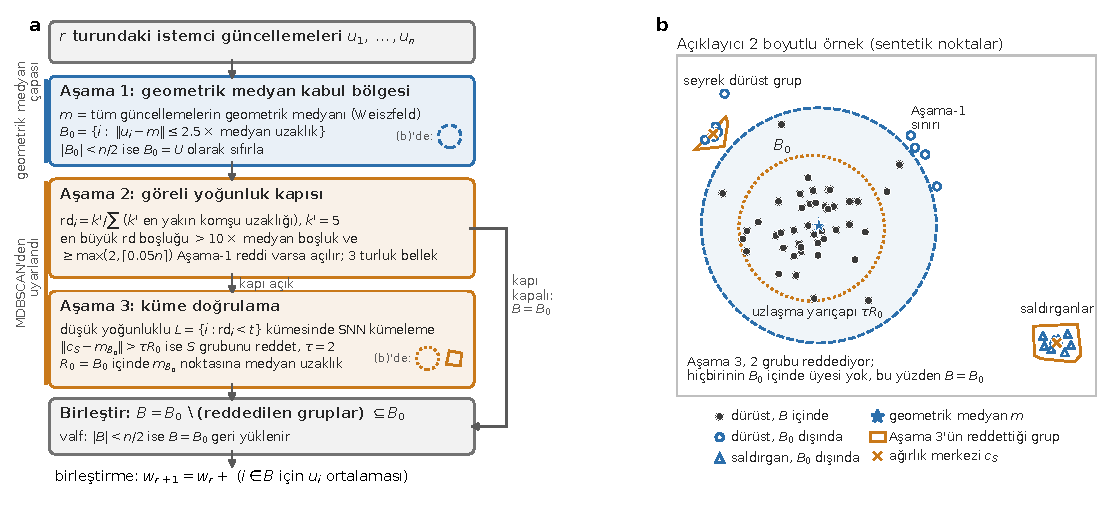
\includegraphics[width=\textwidth]{figures/fed_mdbscan_g_pipeline_tr.pdf}
\caption{\method{} yönteminin karar yolu. (a) Aşama~1 geometrik medyan çevresinde ilk havuz $B_0$'ı oluşturur; Aşama~2 küme aşamasını göreli yoğunluk boşluğu Aşama-1 retleriyle birlikte görüldüğünde açar ve üç turluk bir bellek onu açık tutabilir; Aşama~3 düşük yoğunluklu kümeyi kümeler ve merkezi $B_0$'ın geometrik medyanından $\tau R_0$'dan daha uzak olan grupları reddeder. Son küme her zaman $B\subseteq B_0$ koşulunu sağlar. (b) Kullanılan aşama fonksiyonlarının sentetik noktalar üzerinde ürettiği açıklayıcı iki boyutlu örnek (deney verisi değildir). Aşama~1 saldırganları dokuz dürüst noktayla birlikte dışlar; Aşama~3'ün reddettiği iki grubun tamamı $B_0$ dışında kaldığından küme aşaması kabul kümesini değiştirmez. Örnek yalnızca işleyişi gösterir: Bölüm~\ref{sec:mechanism}'de incelenen kayıtlı saldırılı kontrol noktalarında Aşama~1, $\alpha=0.01$'deki yama saldırısı dışında en fazla birkaç saldırganı dışlar; aynı bölüm her aşamanın ne sıklıkla çalıştığını raporlar.}
\label{fig:pipeline}
\end{figure*}

\method{} yönteminin ilk filtresi (initial filter) şu kümeyi kabul eder:
\begin{equation}
B_0=\{i:\|u_i-m\|_2\leq\rho\operatorname{median}_j\|u_j-m\|_2\},\quad\rho=2.5,
\label{eq:l0}
\end{equation}
burada $m$, geometrik medyanın Weiszfeld yaklaşımıdır. Gönderimlerin yarısından azı kalırsa ilk havuz $U$ olarak sıfırlanır.

$k'=\min(5,n-1)$ için yoğunluk, $k'$ en yakın komşuya olan uzaklıkların toplamı $d_i$ üzerinden hesaplanır. Yerel uygulama $d_i>0$ olduğunda $k'/\max(d_i,10^{-15})$, $d_i=0$ olduğunda $1$ döndürür; tek elemanlı girdi de $1$ döndürür. Kullanılan kapı (deployed gate), sıralı yoğunluk değerleri arasındaki en büyük boşluk (density gap) medyan boşluğun on katını aştığında ve en az $\max(2,\lceil0.05n\rceil)$ gönderim ilk aşamada reddedildiğinde açılır. Üç turluk bir bellek, daha önceki bir etkinleşmeden sonra küme aşamasını (cluster stage) temiz turlarda sönümlenmek kaydıyla etkin tutabilir.

Küme aşaması etkin olduğunda bütün gönderim kümesini yoğunluğa göre bölümler ve düşük yoğunluklu $L$ altkümesi üzerinde paylaşılan komşu kümelemesi çalıştırır. Bulunan her $S$ grubu şu koşulda reddedilir:
\begin{equation}
\begin{gathered}
\|c_S-m_{B_0}\|_2>\tau R_0,\\
R_0=\max\!\left(10^{-10},\operatorname{median}_{j\in B_0}\|u_j-m_{B_0}\|_2\right),
\end{gathered}
\label{eq:consensus}
\end{equation}
burada $c_S$ grubun aritmetik merkezi (arithmetic centroid), $m_{B_0}$ ise $B_0$ kümesinin geometrik medyanıdır ve $\tau=2$ alınır. Bulunan bir gruba atanmamış noktalar bu aşamada test edilmez. Aday gruplar $L\cap B_0$ kümesinden değil $L$ kümesinden oluşturulduğu için $B_0$ dışındaki indeksleri içerebilir.

Birleşik küme, reddedilen grupların üyelerini $B_0$ kümesinden çıkarır. Ardından gönderimlerin yarısından azı kalırsa bir valf (safety valve) $B_0$ kümesini geri yükler. Bu nedenle tam yol monoton bir kaskad olmak zorunda değildir; ancak son çıktı her zaman $B\subseteq B_0$ koşulunu sağlar ve aşağıdaki ilk dışlama sonucunun gerektirdiği yalnızca budur.

\section{Koşullu Analiz}\label{sec:theory}
Bu bölümdeki önermeler tek bir tura ve az önce tanımlanan karar kurallarına ilişkindir. Yalnızca küme içerme, kardinalite ve dışbükeyliğe dayandıkları için ampirik geçerlilikleri, varsayımlarının uygulanan yolda sağlanıp sağlanmadığına bağlıdır; Bölüm~\ref{sec:mechanism} bunu kayıtlı kontrol noktalarında denetler.

\subsection{Kabul kümesi içerme ve kardinalite}
\begin{proposition}[İlk dışlama tabanı / Initial exclusion floor]\label{prop:floor}
$B\subseteq B_0$ ise $\mathrm{FPR}(B)\geq\mathrm{FPR}(B_0)$ olur ve $|A|>0$ için $\mathrm{TPR}(B)\geq\mathrm{TPR}(B_0)$ sağlanır. Bu, monoton bir kaskad ve en fazla $B_0$ kümesini geri yükleyen bir geri dönüş mekanizması için geçerlidir.
\end{proposition}
\begin{IEEEproof}
$H\setminus B_0\subseteq H\setminus B$ ve $A\setminus B_0\subseteq A\setminus B$ içermeleri, ilgili popülasyon boyutlarına bölündükten sonra eşitsizlikleri verir.
\end{IEEEproof}
Dolayısıyla sonraki aşamalar, ilk filtrenin dışladığı dürüst bir istemciyi geri kabul edemez. Yine de çalışma noktasını iyileştirebilirler; örneğin ek dürüst istemci reddetmeden ek saldırganları reddedebilirler. Bu yüzden önerme bir Pareto iyileşmesini dışlamaz. İçerme argümanının kendisi birleşik (conjunctive) kaskadların (cascade) bilinen bir özelliğidir~\cite{viola2004cascade}; burada önemli olan, kullanılan geri dönüş (fallback) mekanizmasının $B_0$ havuzuna içerilmeyi koruyup korumadığıdır.

\begin{corollary}[Sabit kardinaliteli seçim / Fixed-cardinality selection]\label{cor:cardinality}
$n$ gönderimin tam olarak $m$ tanesi kabul ediliyorsa saldırgansız bir turda $\BER=1-m/n$ olur. $a$ saldırgan ve reddedilen $t$ saldırgan varken, $n>a$ koşuluyla $\mathrm{FPR}=(n-m-t)/(n-a)$ olur.
\end{corollary}
\begin{IEEEproof}
Toplam $n-m$ ret vardır; bunların $t$ tanesi saldırgan, $n-m-t$ tanesi dürüsttür.
\end{IEEEproof}
Multi-Krum yapılandırmamız $f=\lceil0.3n\rceil$ ve $m=n-f-2$ kullanır. $n=90$ iken 61 güncelleme tutar; bu yüzden temiz $\BER$ değeri $29/90$ olur. $a=27$ ve $t=0$ iken saldırılı turdaki $\mathrm{FPR}$ değeri $29/63$ olur. Bu özdeşliklerle uyum yalnızca seçim kardinalitesini doğrular (Bölüm~\ref{sec:fidelity}).

\begin{corollary}[Çoğunluk kümesini tutma / Majority-cluster retention]\label{cor:majority}
Saldırgansız bir turda, boyutu $c\geq c_{\min}$ olan tek bir kümeyi tutan kural için $\BER=(n-c)/n\leq(n-c_{\min})/n$ olur. Eşitlik ancak ve ancak $c=c_{\min}$ olduğunda sağlanır. $a$ saldırgan ve $t$ saldırgan reddiyle $\mathrm{FPR}=(n-c-t)/(n-a)$ olur.
\end{corollary}
\begin{IEEEproof}
Küme dışında kalan reddedilmiş indeksleri sayın ve saldırgan retlerini çıkarın.
\end{IEEEproof}
Yerel FLAME yolu $n=90$ iken $c_{\min}=\lfloor n/2\rfloor+1=46$ kullanır; bu da $44/90$ değerinde temiz bir üst sınır verir. Heterojenlik tek başına eşitliği zorunlu kılmaz. Kümelemenin başarısız olduğu veya geri dönüş mekanizmasının devreye girdiği turlar, fiilen yürütülen yola göre ele alınmalıdır.

\subsection{Küme merkezi doğrulaması}
\begin{proposition}[Dışbükey zarf yarıçap sınırı / Convex-hull radius bound]\label{prop:contraction}
Boş olmayan bir $S$ grubu, güncellemelerinin herhangi bir dışbükey birleşimi (convex combination) $g(S)$ ve herhangi bir $m_0$ referansı için
\[
\|g(S)-m_0\|\leq\max_{i\in S}\|u_i-m_0\|
\]
sağlanır. $s$ üyenin düz ortalaması için, bir üyenin yarıçapı en fazla $r_a$, diğerlerininki en fazla $r_b$ ise
\[
\|c_S-m_0\|\leq\frac{r_a+(s-1)r_b}{s}
\]
olur.
\end{proposition}
\begin{IEEEproof}
$g(S)-m_0$ ifadesini $u_i-m_0$ vektörlerinin dışbükey birleşimi olarak yazın ve üçgen eşitsizliğini uygulayın. İkinci ifade $1/s$ ağırlıklarını kullanır.
\end{IEEEproof}
Buna göre bir grup merkezi bir topun dışındaysa en az bir üye de dışındadır. Bu ifade tek tek üyelere değil gruba ilişkindir. Bütün bir grubu reddetmek topun içindeki üyeleri de dışlayabilir: gerçel doğru üzerinde merkez 0 ve yarıçap 2 iken $\{1,5\}$ grubunun merkezi 3'tür; üyesi 1 topun içinde olduğu hâlde grup reddedilir. Tersine, sapmalar birbirini götürerek bir üye dışarıdayken merkezi topun içine yerleştirebilir. İlk filtre ve uzlaşma filtresi (consensus filter) de farklı referans noktaları ve yarıçaplar kullanır; bu nedenle sınır, bu iki filtrenin istemci düzeyindeki kararlarını sıralamaz.

\begin{proposition}[Küme merkezi doğrulamasının etkisiz kalması için yeter koşul / Sufficient condition for inactive centroid validation]\label{prop:vacuity}
Boş olmayan $B_0$ için
\[
\Gamma(B_0)=\frac{\max_{i\in B_0}\|u_i-m_{B_0}\|_2}{R_0}
\]
tanımlansın; burada $R_0$, \eqref{eq:consensus} içindeki tabanlı yarıçaptır (floored radius). $\Gamma(B_0)\leq\tau$ ise boş olmayan hiçbir $S\subseteq B_0$ grubu \eqref{eq:consensus} ile reddedilmez. Test edilen her grup böyle bir altkümeyse ve başka hiçbir aşama üye çıkarmıyorsa son kabul kümesi $B=B_0$ olur.
\end{proposition}
\begin{IEEEproof}
$B_0$ kümesinin her üyesi $m_{B_0}$ merkezli, $\tau R_0$ yarıçaplı kapalı topun içindedir. Top dışbükey olduğundan bir $S\subseteq B_0$ altkümesinin üyelerinin her dışbükey birleşimi topun içindedir ve kesin ret eşitsizliği sağlanamaz.
\end{IEEEproof}
Koşul yeterlidir ama gerekli değildir. Ayrıca aday grupları $B_0$ dışındaki üyeleri içerebilen bileşik yöntemimiz için genel olarak geçerli değildir. Örneğin $B_0=\{-1,1\}$ için $\Gamma=1$ olur; ama $\{1,10\}$ grubunun merkezi $5.5$ olduğundan grup yarıçap-2 testini geçemez. Bu yüzden önermeyi kayıtlı matrislere uygulamadan önce altküme koşulunu doğruluyoruz.

\subsection{Yoğunluk sıralaması ve uygulama sınırı}
\begin{proposition}[Ayırıcı eşikle yoğunluk ayrımı / Density separation with a separating threshold]\label{prop:density}
Uzaklık toplamlarının kesinlikle pozitif olduğu ideal $\rd(i)=k'/d_i$ skorunu ele alalım. $|A|\geq k'+1$ olsun; bütün saldırgan çiftleri arasındaki uzaklıklar en fazla $\delta_A>0$ ve her dürüst noktanın ortalama $k'$-en yakın komşu uzaklığı en az $\delta_H>\delta_A$ olsun. O zaman
\[
\min_{a\in A}\rd(a)\geq1/\delta_A>1/\delta_H\geq\max_{i\in H}\rd(i)
\]
olur. $\max_{i\in H}\rd(i)<t\leq\min_{a\in A}\rd(a)$ koşulunu sağlayan bir eşik için $L=\{i:\rd(i)<t\}$ kümesi bütün dürüst noktaları içerir ve hiçbir saldırgan noktayı içermez.
\end{proposition}
\begin{IEEEproof}
Her saldırganın $\delta_A$ uzaklık içinde $k'$ başka saldırganı vardır; bu nedenle en yakın komşu uzaklık toplamı en fazla $k'\delta_A$ olur. Varsayılan dürüst ortalama uzaklık $d_i\geq k'\delta_H$ verir. Terslerini almak sıralamayı, eşik koşulu da seçilen kümeyi verir.
\end{IEEEproof}
Eşik kısıtı zorunludur, çünkü bütün skorların üzerindeki bir eşik saldırganları da seçer. Uygulamanın bir sınır durumu da vardır: etkin en yakın komşu uzaklıklarının toplamı tam olarak sıfır olduğunda kod $\rd=1$ döndürür; $k'=1$ ile tek boyutlu $[0,0,0.1,0.2]$ girdisi için gerçek çıktı $[1,1,10,10]$ olur. Ancak kayıtlı yüksek boyutlu matrislerde en yakın komşu araması, bit düzeyinde özdeş güncellemeler (exact duplicates) arasında bile küçük pozitif uzaklıklar döndürür; bu yüzden bu dal orada hiç çalışmaz (Bölüm~\ref{sec:mechanism}). Kümeleme sezgisi önceki gözlemlerle uyumludur~\cite{bellachia2026sok}; ancak belirli bir koşumu (run) açıklamak, o koşumda hesaplanan skorları ve yönlendirme (routing) kararlarını gerektirir.

\subsection{Koşullu bir skor sıralaması sonucu}
\begin{theorem}[Yalnız dürüst ret / Honest-only rejection]\label{thm:inversion}
$H$ ve $A$ boş olmasın ve $1\leq k\leq|H|$ olsun. Bir kural en yüksek $k$ skoru atıyorsa ve $s^H_{(k)}$ en büyük $k$'ıncı dürüst skor olmak üzere $\max_{a\in A}s_a<s^H_{(k)}$ ise
\[
\mathrm{TPR}=0,\quad\mathrm{FPR}=k/|H|,\quad J=-k/|H|
\]
olur. Eşik kuralı için, $\rho\geq\max_{a\in A}s_a$ ise aynı sonuç $k=|\{i\in H:s_i>\rho\}|>0$ ile geçerlidir.
\end{theorem}
\begin{IEEEproof}
Kesin sıralama, atılan $k$ indeksin hepsini $H$ içine yerleştirir. Eşik durumunda hiçbir saldırgan eşiği aşmaz. Dürüst ve saldırgan retlerini sayın.
\end{IEEEproof}
Teorem koşullu bir sayma sonucudur. Min-Max ve Min-Sum uzaklıkları kısıtlar~\cite{shejwalkar2021}, ancak bu kısıtlar teoremin sıralama öncülünü her skor için sağlamaz. Örneğin $\{-2,0,0.1,2\}$ dürüst noktalarının en büyük ikili uzaklığı 4'tür ve $-1$ noktası her birine en fazla 3 uzaklıktadır; yine de dürüst geometrik medyana en uzak üç noktayı reddeden bir kural, $-2$ ve $2$ ile birlikte $-1$ noktasını da reddeder. Negatif $J$ ayrıca model doğruluğu veya saldırı başarısı hakkında doğrudan bir şey söylemez. Ret bütçesini büyütmek $J$ değerini ancak yalnız dürüst sıralaması korunduğu sürece daha negatif yapar.

Ne içerme ne de dışbükeylik sonucu referans noktasının nasıl elde edildiğine bağlıdır; bu nedenle ikisi de güvenilir sunucu verisi kullanan kurallara uygulanır. FLTrust'ın Bölüm~\ref{sec:attack} içinde elde ettiği pozitif aile ortalaması $J$ ampirik bir gözlemdir; dış bir referansın dayanıklılık (robustness) için gerekli ya da yeterli olduğunu göstermez.

\section{Deney Protokolü}\label{sec:protocol}
\begin{table}[!t]
\centering\footnotesize
\setlength{\tabcolsep}{4pt}
\caption{Bloklara Göre Planlanan Değerlendirme Kapsamı}\label{tab:coverage}
\begin{adjustbox}{max width=\columnwidth}
\begin{tabular}{lr}
\toprule
Blok & Birim \\
\midrule
Ana matris (saldırılı ve saldırgansız) & 1500 \\
Ablasyon varyantları & 252 \\
Eşleşen saldırısı kapatılmış kontroller & 156 \\
Kâhin (oracle) tanıları & 78 \\
Alternatif bölümleme politikası & 54 \\
Sabit yerel adım kontrolü & 54 \\
Saldırı başlangıç/bitiş zamanlaması & 36 \\
Planlanan toplam & 2130 \\
\bottomrule
\end{tabular}
\end{adjustbox}

\par\vspace{3pt}\parbox{\linewidth}{\footnotesize Bir birim, bir kural--koşul--tohum koşumudur. Planlanan 2130 birimin 2125'i tamamlanmış, 5'i doldurulmak ya da yeni tohumla tekrarlanmak yerine başarısız olarak tutulmuştur. Bloklar dengeli bir tam faktöriyel tasarım oluşturmaz.}
\end{table}


\begin{table}[!t]
\centering\footnotesize
\setlength{\tabcolsep}{4pt}
\caption{Deney Düzeni}\label{tab:setup}
\begin{tabular}{@{}lp{0.64\columnwidth}@{}}
\toprule
Öğe & Ayar \\
\midrule
MNIST, Fashion-MNIST & çok katmanlı algılayıcı 784--200--10 \\
UCI HAR & çok katmanlı algılayıcı 561--128--64--6, dropout 0.2 \\
CIFAR-10 & iki evrişim katmanı (32, 64 kanal) ve tam bağlantılı katmanlar 256--10 \\
\addlinespace[2pt]
İstemciler & 100; turda 90, saldırganlar her turda \\
Eğitim & 30 tur, 3 yerel epok, mini-batch boyutu 32 \\
Optimizasyon & öğrenme oranı 0.01, momentum 0.9 \\
Tohumlar & 42, 137, 2024 \\
Bölümleme & Dirichlet, $\alpha\in\{0.5,0.1,0.01\}$; log-normal tutma, $\sigma=0.5$; istemci başına $\geq20$ örnek \\
Kök kümesi & 100 örnek, bütün kurallar için ayrılır \\
Yazılım & Python 3.12, PyTorch 2.11, CUDA \\
\bottomrule
\end{tabular}
\end{table}

\subsection{Simülasyon ve kayıtlar}
Bütün deneyler PyTorch ile yazılmış bir federe öğrenme simülasyonunda (simulation) çalışır: her turda çizelgedeki istemciler tek bir süreç içinde art arda eğitilir ve güncellemeleri sunucu tarafı kurala iletilir. İletişim, gecikme ve cihazların hesaplama gücü modellenmez. Kurulum, cihazlar arası ve Nesnelerin İnterneti kurulumlarını verisi üzerinden yansıtır: IID olmayan bölümlemeler, eşit olmayan istemci veri miktarları, kısmi katılım ve bir akıllı telefon sensörü veri kümesi (UCI HAR~\cite{anguita2013har}). PyTorch'un deterministik kipi (deterministic mode) kapalıydı; bu yüzden GPU sonuçlarının bit düzeyinde aynen tekrarlanması gerekmez. Her koşum her tur için çizelgedeki, katılan, kabul edilen ve reddedilen kimlikleri, bunlardan çıkan karışıklık sayılarını, test doğruluğunu ve yama saldırısının başarısını, bölümlemenin, çizelgenin ve başlangıç modelinin özetleriyle (hash) birlikte kaydeder. Bölüm~\ref{sec:benign} ve~\ref{sec:attack}'deki tablolar bu kayıtlardan hesaplanır.

\subsection{Veri, eğitim ve kapsam}
Deneylerde herkese açık dört veri kümesi kullanılır: MNIST~\cite{lecun1998}, Fashion-MNIST~\cite{xiao2017fmnist}, UCI HAR~\cite{anguita2013har} ve CIFAR-10~\cite{krizhevsky2009}. Tablo~\ref{tab:setup} modelleri ve eğitim ayarlarını özetler. Eğitim örnekleri istemcilere bir Dirichlet çekilişiyle dağıtılır~\cite{hsu2019}. Ardından her istemci kendi payının rastgele bir $\min(1,e^{Z})$, $Z\sim\mathcal{N}(0,0.5^2)$, oranını tutar (log-normal tutma, lognormal retention), ancak mümkün olduğunda en az 20 örnek korunur; atılan örnekler başka istemcilere verilmez. Sonra bütün istemci verilerinden tekdüze olarak çekilen 100 örnek, her kural için FLTrust kök kümesi (root set) olarak ayrılır; böylece belirli bir tohumda bütün kurallar aynı istemci verisini görür. Son olarak en az örnek onarımı (minimum-count repair), her istemcide en az 20 örnek olana kadar en büyük istemcilerden örnek taşır. Tohumlu bir çizelge her turda 100 istemciden 90'ını seçer; saldırganların kimlikleri sabittir ve her tura katılırlar, her dürüst istemci ise turların rastgele bir alt kümesine katılır. MNIST, Fashion-MNIST ve UCI HAR 17 koşullu ortak bir ana bloğu paylaşır; CIFAR-10'un kapsamı daha dardır. Arşivlenmiş değerlendirme 149 iş ve 2\,130 planlı kural--koşul--tohum biriminden oluşur (Tablo~\ref{tab:coverage}); bunların 2\,125'i tamamlanmıştır. Beş başarısızlık, yani dört örnek ağırlıklı HAR koşumu ve Min-Max altındaki bir CIFAR FLAME koşumu, hesapta tutulmuş; ne doldurulmuş ne de yenisiyle değiştirilmiştir. Bu revizyon için 39 kanonik koşum yeniden yürütülmüş ve 36 kontrol koşumu eklenmiştir; bunlar ayrı raporlanır ve arşivlenmiş toplamları değiştirmez (ek belge).

\subsection{Kontrol blokları ve saldırılar}
Saldırgansız ana koşullar üç yoğunlaşma değerinin her birinde sıfır kötü niyetli istemciyle yapılandırılmıştır; CIFAR için $\alpha=0.5$ kontrol hücresi yoktur. Yama arka kapısı karşılaştırması için saldırısı kapatılmış kontroller, saldırılı yapılandırmaların istemci kimliklerini ve çizelgelerini korur ve yalnızca saldırıyı kapatır. Tablo~\ref{tab:coverage}'deki oracle, alternatif bölümleme, sabit adım ve zamanlama blokları, raporlanan tabloların dışında kalan tanı bloklarıdır: oracle koşumları etkin saldırganları birleştirmeden önce çıkarır, alternatif bölümleme onarımı uygulamaz, sabit adım kontrolü yerel eğitimi beş optimizasyon adımıyla sınırlar, zamanlama bloğu ise yalnızca 10 ile 19. turlarda saldırır.

Beş saldırı ailesi şunlardır: yüksek Gauss gürültüsü (koordinat başına standart sapma 5), etiket çevirme, sağ alt köşede $3\times3$ beyaz yama arka kapısı (hedef sınıf 0, zehirleme oranı $0.2$), sınırlı rastgele bozulmalar ve kısıtlı her şeyi bilen yoklamalar. Sınırlı aile, $0.005$ göreli ölçekte bir yön yoklamasını ve $0.3$ göreli ölçekte rastgele gürültüyü içerir; ikincisi kodda eski \texttt{adaptive\_gaussian} adını taşır, ancak eniyilenmiş bir uyarlanabilir saldırı değildir. Kısıtlı yoklamalar, dürüst ortalamanın tersi yönünde, Min-Max veya Min-Sum sınırını sağlayacak biçimde ölçeklenmiş ortak bir vektör gönderir~\cite{shejwalkar2021}.

\subsection{Uygulamalar}\label{sec:fidelity}
Panel düz ortalama, örnek ağırlıklı ortalama, norm kırpma, koordinat bazında medyan, $f=\lceil0.3n\rceil$ ve $m=n-f-2$ ile Multi-Krum, 100 kök örnekli normalize FLTrust, $0.001$ gürültü düzeyli yerel HDBSCAN tabanlı bir FLAME ve \method{} ile yedi ablasyon varyantından oluşur. Yerel FLTrust kuralını, yazarların gösterim kodundaki kuralın bir aktarımıyla 18 kayıtlı matris üzerinde karşılaştırdık; göreli fark $2.8\times10^{-7}$'nin altında kaldı. Bölüm~\ref{sec:mechanism}'deki beş adımlı Min-Max kontrol noktası matrislerinin altısında yerel Multi-Krum skorları yayımlanmış kuralla~\cite{blanchard2017} örtüşür; seçimler yalnızca özdeş saldırgan kopyaları arasındaki eşitliklerin nasıl bozulduğunda ayrışır ve bu, birleştirilmiş güncellemeyi float32 hassasiyetinde değiştirmez. FLAME'in kırpma, ortalama alma ve gürültü ölçekleme adımları da sunucunun birleştirme yolu üzerinden sınandı. Tamamlanmış 200 FLAME koşumunun hepsinde (6\,000 tur) kaydedilmiş kabul kimliklerini saydık; Bölüm~\ref{sec:benign}'da kullanılan tutulan küme boyutları bu sayımdan gelir. Bu denetimlerin kapsamı ek belgede ayrıntılı olarak verilmiş, Bölüm~\ref{sec:limits}'da özetlenmiştir.

\subsection{Ölçütler}
Dürüst fayda kaybı, aynı saldırgansız koşulda düz ortalamanın son doğruluğu eksi savunmanın son doğruluğudur; saldırı altında fayda, savunmanın doğruluğu eksi düz ortalamanın doğruluğudur. Doğruluk karşılaştırmaları her hücrenin tamamlanmış tohumlarını kullanır. Ayrıca saldırgan yakalama oranını, dürüst ret oranını, $J$ değerini ve tetiklenmiş hedef dışı örneklerdeki saldırı başarı oranını (ASR) raporluyoruz. FLTrust güveni pozitif olmayan gönderimlere sıfır ağırlık verir; BER, FPR ve TPR değerleri bu sıfır ağırlık kararlarını sayar. Alarm özgüllüğü yalnızca bileşik yöntem için raporlanır; paneldeki kurallar içinde tur düzeyinde alarm üreten tek yöntem odur.

\section{Saldırgansız Dışlama ve Fayda}\label{sec:benign}
\begin{table*}[!tp]
\centering\footnotesize
\setlength{\tabcolsep}{4pt}
\caption{Saldırgansız Dürüst İstemci Dışlama Oranı (BER, \%)}\label{tab:ber}
\begin{adjustbox}{max width=\textwidth}
\begin{tabular}{lrrrrrrrrrrr}
\toprule
& \multicolumn{3}{c}{$\alpha=0.5$} & \multicolumn{4}{c}{$\alpha=0.1$} & \multicolumn{4}{c}{$\alpha=0.01$} \\
\cmidrule(lr){2-4}\cmidrule(lr){5-8}\cmidrule(lr){9-12}
Kural & MNIST & Fashion & HAR & MNIST & Fashion & HAR & CIFAR-10 & MNIST & Fashion & HAR & CIFAR-10 \\
\midrule
Düz ortalama (savunmasız) & 0.0 & 0.0 & 0.0 & 0.0 & 0.0 & 0.0 & 0.0 & 0.0 & 0.0 & 0.0 & 0.0 \\
Örnek ağırlıklı ortalama (savunmasız) & 0.0 & 0.0 & 0.0 & 0.0 & 0.0 & 0.0 & -- & 0.0 & 0.0 & 0.0 & -- \\
Norm kırpma & 0.0 & 0.0 & 0.0 & 0.0 & 0.0 & 0.0 & -- & 0.0 & 0.0 & 0.0 & -- \\
Koordinat bazında medyan & 0.0 & 0.0 & 0.0 & 0.0 & 0.0 & 0.0 & -- & 0.0 & 0.0 & 0.0 & -- \\
Multi-Krum & 32.2 & 32.2 & 32.2 & 32.2 & 32.2 & 32.2 & -- & 32.2 & 32.2 & 32.2 & -- \\
FLTrust (normalize) & 33.1 & 31.9 & 11.9 & 25.3 & 27.3 & 19.6 & -- & 30.3 & 32.3 & 31.0 & -- \\
FLAME (HDBSCAN) & 48.9 & 48.9 & 48.3 & 48.9 & 48.7 & 47.4 & 48.7 & 48.7 & 47.0 & 42.4 & 45.5 \\
Fed-MDBSCAN-G (tam) & 0.3 & 0.4 & 2.1 & 0.2 & 0.5 & 24.1 & 0.1 & 42.6 & 38.7 & 24.4 & 39.9 \\
\bottomrule
\end{tabular}
\end{adjustbox}

\par\vspace{3pt}\parbox{\linewidth}{\footnotesize Hiç saldırgan yokken reddedilen dürüst istemci--tur gönderimleri; üç tohum, 30 tur ve turda 90 katılımcı (hücre başına 8\,100 dürüst istemci--tur). Fashion, Fashion-MNIST anlamına gelir; tireler planlanan kapsam dışındaki koşullardır. FLTrust sıfır ağırlıklı gönderimleri sayar. Norm kırpma ve koordinat bazında medyan hiçbir istemciyi reddetmez; bu yüzden BER değerleri tanım gereği sıfırdır ve dürüst maliyetleri Tablo~\ref{tab:buc} içinde görülür.}
\end{table*}

\begin{table*}[!tp]
\centering\footnotesize
\setlength{\tabcolsep}{4pt}
\caption{Saldırgansız Dürüst Fayda Kaybı (BUC, Yüzde Puan)}\label{tab:buc}
\begin{adjustbox}{max width=\textwidth}
\begin{tabular}{lrrrrrrrrrrr}
\toprule
& \multicolumn{3}{c}{$\alpha=0.5$} & \multicolumn{4}{c}{$\alpha=0.1$} & \multicolumn{4}{c}{$\alpha=0.01$} \\
\cmidrule(lr){2-4}\cmidrule(lr){5-8}\cmidrule(lr){9-12}
Kural & MNIST & Fashion & HAR & MNIST & Fashion & HAR & CIFAR-10 & MNIST & Fashion & HAR & CIFAR-10 \\
\midrule
Norm kırpma & 0.0 & 0.0 & $+$0.2 & 0.0 & 0.0 & $+$2.2 & -- & $+$22.5 & $+$13.3 & 0.0 & -- \\
Koordinat bazında medyan & $+$0.6 & $+$0.8 & $+$9.8 & $+$4.7 & $+$5.1 & $+$33.3 & -- & $+$64.4 & $+$40.9 & $+$23.8 & -- \\
Multi-Krum & $+$1.0 & $+$1.3 & $+$2.8 & $+$4.6 & $+$4.8 & $+$29.2 & -- & $+$44.9 & $+$33.6 & $+$11.0 & -- \\
FLTrust (normalize) & $+$2.4 & $+$2.5 & $+$13.2 & $+$3.3 & $+$4.1 & $+$29.2 & -- & $+$11.6 & $+$5.1 & $+$10.6 & -- \\
FLAME (HDBSCAN) & $+$1.7 & $+$1.9 & $+$19.6 & $+$10.4 & $+$6.7 & $+$38.1 & $+$15.5 & $+$65.5 & $+$45.9 & $+$15.2 & $+$15.6 \\
Fed-MDBSCAN-G (tam) & 0.0 & 0.0 & $+$1.8 & 0.0 & $+$0.1 & $+$26.8 & 0.0 & $+$59.2 & $+$41.9 & $+$10.4 & $+$14.9 \\
\bottomrule
\end{tabular}
\end{adjustbox}

\par\vspace{3pt}\parbox{\linewidth}{\footnotesize Savunmasız düz ortalamanın son tur doğruluğu eksi savunmanınki; Tablo~\ref{tab:ber} ile aynı koşumlar. Pozitif değerler düz ortalamadan daha düşük doğruluğu gösterir. Üç tohum üzerinden ortalamalar; tohum başına aralıklar ek belgede verilmiştir.}
\end{table*}

\begin{table}[!t]
\centering\footnotesize
\setlength{\tabcolsep}{4pt}
\caption{Saldırgansız Koşullarda FLAME'in Tuttuğu Küme Boyutları}\label{tab:flame_sizes}
\begin{adjustbox}{max width=\columnwidth}
\begin{tabular}{llrrr}
\toprule
Veri kümesi & $\alpha$ & Ort. boyut & Aralık & Boyut 46 \\
\midrule
MNIST & 0.5 & 46.01 & 46--47 & 89/90 \\
MNIST & 0.1 & 46.03 & 46--47 & 87/90 \\
MNIST & 0.01 & 46.17 & 46--49 & 77/90 \\
Fashion & 0.5 & 46.01 & 46--47 & 89/90 \\
Fashion & 0.1 & 46.19 & 46--50 & 81/90 \\
Fashion & 0.01 & 47.73 & 46--56 & 39/90 \\
HAR & 0.5 & 46.50 & 46--53 & 67/90 \\
HAR & 0.1 & 47.30 & 46--51 & 38/90 \\
HAR & 0.01 & 51.83 & 46--62 & 9/90 \\
CIFAR-10 & 0.1 & 46.13 & 46--48 & 79/90 \\
CIFAR-10 & 0.01 & 49.09 & 46--61 & 64/90 \\
\bottomrule
\end{tabular}
\end{adjustbox}

\par\vspace{3pt}\parbox{\linewidth}{\footnotesize Saldırgansız ana hücrelerde kaydedilmiş kabul kimliklerinden sayılmıştır; her satır üç tohum ve 90 tur kapsar. Boyut 46, izin verilen en küçük boyuttur: $\lfloor n/2\rfloor+1$.}
\end{table}

\begin{table}[!t]
\centering\footnotesize
\setlength{\tabcolsep}{4pt}
\caption{$\alpha=0.01$'de Saldırgansız Son Doğruluk (\%): Kurallar ve Aynı Büyüklükte Rastgele Altkümeler}\label{tab:random}
\begin{adjustbox}{max width=\columnwidth}
\begin{tabular}{lrrrrr}
\toprule
Veri kümesi & FedAvg & Multi-Krum & Multi-Krum & FLAME & FLAME \\
 &  & kural & rastgele & kural & rastgele \\
\midrule
MNIST & 85.65 & 40.71 & 84.36 & 20.10 & 44.65 \\
Fashion & 73.63 & 40.04 & 72.58 & 27.74 & 41.86 \\
HAR & 45.53 & 34.57 & 50.44 & 30.35 & 37.50 \\
\bottomrule
\end{tabular}
\end{adjustbox}

\par\vspace{3pt}\parbox{\linewidth}{\footnotesize Üç tohum üzerinden ortalamalar; Fashion, Fashion-MNIST demektir. Rastgele altkümeler her turda kuralın seçtiklerinin yerini alır ve kabul sayısını korur: Multi-Krum için 61, FLAME için kanonik koşumun o turdaki sayısı. Kırpma ve gürültü kuralları korunur; eşleştirilmiş farklar ek belgededir.}
\end{table}


Hiç saldırgan yokken bile ret yapan kurallar birçok koşulda dürüst gönderimlerin büyük bir kısmını dışlar (Tablo~\ref{tab:ber}, Şekil~\ref{fig:ber}). Multi-Krum, mevcut dokuz hücrenin hepsinde, Sonuç~\ref{cor:cardinality}'in gerektirdiği gibi tam olarak \%32.22 dışlar.

FLAME'in temiz dışlamasını küme boyutu kuralı sınırlar ve temiz turların çoğunda FLAME bu sınıra ulaşır. 990 turun 719'unda izin verilen en küçük çoğunluğu, yani 90 güncellemenin tam 46'sını tutar (Tablo~\ref{tab:flame_sizes}); hücre düzeyindeki dışlaması \%42.4 ile \%48.9 arasındadır. Güçlü heterojenlik altında, en belirgin olarak HAR'da, daha büyük kümeler tutar ve sınıra daha seyrek ulaşır; dolayısıyla gerçekleşen dışlama veriye de bağlıdır.

\method{} farklı davranır. Dışlaması $\alpha=0.5$'te \%2.1'in altında kalır, ancak $\alpha=0.01$'de \%42.6'ya ulaşır (Tablo~\ref{tab:ber}); çünkü Aşama-1 eşiği her turun medyan yarıçapıyla ölçeklenir ve kabul edilen oran bu dağılımın biçimini izler.

Dışlama fayda kaybının yalnızca bir kaynağıdır (Tablo~\ref{tab:buc}). Koordinat bazında medyan hiçbir istemciyi reddetmez, yine de MNIST'te $\alpha=0.01$ koşulunda son doğruluğu düz ortalamanın 64.4 yüzde puan altındadır; en büyük kayıp olan 65.55 puan, aynı koşulda FLAME'e aittir. Raporlanan hücreler üzerinden ortalandığında kayıp, $\alpha$ 0.5'ten 0.01'e düştükçe 3.3'ten 27.5 puana çıkar; bu yüzden kabul oranları tek başına dürüst faydayı değerlendirmeye yetmez. $\alpha=0.01$'deki Multi-Krum için hangi güncellemelerin tutulduğu, kaç güncellemenin tutulduğundan daha önemlidir (Tablo~\ref{tab:random}): seçtiği 61 güncellemeyi aynı büyüklükte rastgele bir altkümeyle değiştirmek son doğruluğu ortalamada 15.9 ile 43.7 puan artırır ve MNIST ile Fashion-MNIST'te tekdüze ortalamanın 1.3 puan yakınına getirir. FLAME'de her turda kanonik kabul sayısıyla eşleştirilmiş rastgele bir altküme, doğruluğu her tohum çiftinde 7.2 ile 24.6 puan artırır; gürültüyü kaldırmak ise doğruluğu en fazla 0.33 puan değiştirir. Tekdüze ortalamaya kalan 8.0 ile 41.0 puanlık fark FLAME'in kırpmasını, daha küçük kabul kümesini ya da her ikisini yansıtır.

\begin{figure}[!t]
\centering
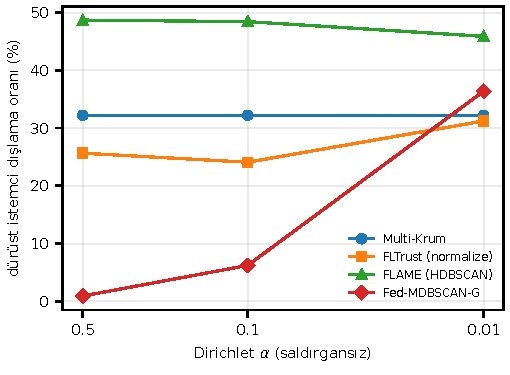
\includegraphics[width=\columnwidth]{figures/ber_vs_alpha_tr.pdf}
\caption{Mevcut veri kümesi hücreleri üzerinden ortalanmış saldırgansız dışlama. Kapsam yoğunlaşma değerine ve yönteme göre değişir. FLTrust sıfır ağırlıklı gönderimleri sayar. FLAME sınırına her turda ulaşılması gerekmez; doğrudan boyutlar Tablo~\ref{tab:flame_sizes} içindedir.}\label{fig:ber}
\end{figure}

Bileşik yöntemin tur düzeyindeki alarmı güçlü heterojenlik altında düşük özgüllüğe sahiptir (ek belge): $\alpha=0.01$'de her veri kümesindeki her saldırgansız turda, $\alpha=0.1$'de ise HAR'daki 90 turun 89'unda alarm üretir. Bu alarmların hepsi yanlıştır.

\section{Saldırı Altında Ayırt Etme}\label{sec:attack}
\begin{table}[!t]
\centering\footnotesize
\setlength{\tabcolsep}{4pt}
\caption{Saldırı Ailesine Göre İstemci Düzeyinde Ayırt Etme}\label{tab:discrimination}
\begin{adjustbox}{max width=\columnwidth}
\begin{tabular}{lrrrrr}
\toprule
Saldırgan ailesi & Hücre & TPR & FPR & $J$ & Fayda \\
 &  & (\%) & (\%) & (yp) & (yp) \\
\midrule
Yüksek Gauss gürültüsü ($\sigma=5$) & 60 & 87.5 & 18.9 & $+$68.6 & $+$13.7 \\
Etiket çevirme & 36 & 69.7 & 24.8 & $+$45.0 & $-$9.0 \\
Yama arka kapısı & 16 & 34.0 & 32.3 & $+$1.8 & $-$19.2 \\
Sınırlı rastgele yön & 72 & 34.1 & 33.7 & $+$0.4 & $-$23.0 \\
Kısıtlı her şeyi bilen & 28 & 21.8 & 38.0 & $-$16.1 & $-$10.6 \\
\bottomrule
\end{tabular}
\end{adjustbox}

\par\vspace{3pt}\parbox{\linewidth}{\footnotesize $J=\mathrm{TPR}-\mathrm{FPR}$ (Youden indeksi); $J<0$ dürüst istemcilerin saldırganlardan önce reddedildiğini gösterir. Fayda, aynı koşulda savunmanın doğruluğu eksi savunmasız doğruluktur. Her satır, ret yapan dört kuralın kural~$\times$~veri kümesi~$\times$~koşul hücrelerini birleştirir; ailelerin kapsamı farklı olduğundan satırlar betimsel ortalamalardır.}
\end{table}

\begin{table}[!t]
\centering\footnotesize
\setlength{\tabcolsep}{4pt}
\caption{Kısıtlı Her Şeyi Bilen Saldırgan Altında Çalışma Noktaları}\label{tab:constrained}
\begin{adjustbox}{max width=\columnwidth}
\begin{tabular}{llrrrr}
\toprule
Veri kümesi & Kural & TPR & FPR & $J$ & Öngörülen \\
 &  & (\%) & (\%) & (yp) & FPR (\%) \\
\midrule
\multicolumn{6}{l}{\emph{$\alpha=0.1$}} \\
\quad MNIST & Multi-Krum & 0.00 & 46.03 & $-$46.03 & 46.03 \\
\quad MNIST & FLAME (HDBSCAN) & 0.00 & 68.11 & $-$68.11 & $\leq69.84$ \\
\quad Fashion & Multi-Krum & 0.00 & 46.03 & $-$46.03 & 46.03 \\
\quad Fashion & FLAME (HDBSCAN) & 0.00 & 65.59 & $-$65.59 & $\leq69.84$ \\
\quad HAR & Multi-Krum & 57.90 & 21.22 & $+$36.68 & 46.03 \\
\quad HAR & FLAME (HDBSCAN) & 96.67 & 27.25 & $+$69.42 & $\leq69.84$ \\
\quad CIFAR-10 & FLAME (HDBSCAN) & 8.33 & 62.94 & $-$54.60 & $\leq69.84$ \\
\addlinespace[3pt]
\multicolumn{6}{l}{\emph{$\alpha=0.01$}} \\
\quad MNIST & Multi-Krum & 0.00 & 46.03 & $-$46.03 & 46.03 \\
\quad MNIST & FLAME (HDBSCAN) & 0.00 & 58.82 & $-$58.82 & $\leq69.84$ \\
\quad Fashion & Multi-Krum & 0.00 & 46.03 & $-$46.03 & 46.03 \\
\quad Fashion & FLAME (HDBSCAN) & 0.00 & 63.19 & $-$63.19 & $\leq69.84$ \\
\quad HAR & Multi-Krum & 0.00 & 46.03 & $-$46.03 & 46.03 \\
\quad HAR & FLAME (HDBSCAN) & 0.00 & 59.47 & $-$59.47 & $\leq69.84$ \\
\quad CIFAR-10 & FLAME (HDBSCAN) & 0.00 & 57.51 & $-$57.51 & $\leq69.84$ \\
\bottomrule
\end{tabular}
\end{adjustbox}

\par\vspace{3pt}\parbox{\linewidth}{\footnotesize Yüzde otuz saldırgan: turda 63 dürüst ve 27 saldırgan katılımcı. Öngörülen FPR, sıfır saldırgan yakalamadaki ($\mathrm{TPR}=0$) değerdir: Multi-Krum için bir özdeşlik, FLAME için bir üst sınır (Sonuç~\ref{cor:cardinality}--\ref{cor:majority}). FLTrust ve Fed-MDBSCAN-G böyle bir öngörü vermez; kural bazındaki oranları ek belgededir. CIFAR-10/FLAME/$\alpha=0.1$ (iki tamamlanmış tohumdan 60 tur) dışında her hücrede 90 kayıtlı tur vardır.}
\end{table}


Saldırıları ayırt etme başarımı büyük ölçüde saldırı ailesine bağlıdır (Tablo~\ref{tab:discrimination}; kural bazında ek belgede). Ret yapan dört kural üzerinden ortalandığında $J$, yüksek Gauss gürültüsünde $+68.6$ puandan başlayıp etiket çevirmeden geçerek yama arka kapıları ve sınırlı bozulmalarda sıfıra yakın değerlere iner, kısıtlı yoklamalarda ise negatif olur ($-16.1$). Aileler saldırgan oranı, yoğunlaşma ve veri kümesi kapsamı bakımından da farklı olduğundan bu sıralama betimseldir.

Kısıtlı yoklamalar altında Multi-Krum altı hücresinin beşinde yalnızca dürüst istemcileri reddeder (Tablo~\ref{tab:constrained}). Bu hücrelerin her birinde $2\,610$ retin hepsi dürüsttür; bu da Sonuç~\ref{cor:cardinality}'in sıfır saldırgan yakalamada öngördüğü $\mathrm{FPR}=29/63=46.03\%$ değerini verir. İstisna, saldırgan yakalamanın pozitif olduğu HAR, $\alpha=0.1$ hücresidir ($J=+36.68$ puan). Kısıtlı saldırganların hepsi aynı vektörü gönderdiğinden sıfır yakalama, seçim sınırındaki eşitliklerin nasıl bozulduğundan da kaynaklanabilir; dolayısıyla bu sayımlar Teorem~\ref{thm:inversion}'in sıralama öncülünü tek başına kanıtlamaz.

FLAME de benzer davranır. Sekiz kısıtlı yoklama hücresinin altısında saldırgan yakalaması sıfırdır ve FPR \%57.51 ile \%68.11 arasındadır; bu değerler, hiçbir saldırgan reddedilmediğinde tutulan çoğunluğun getirdiği $44/63=69.84\%$ tavanının altındadır. \method{} de bu hücrelerin birçoğunda düşük veya sıfır saldırgan yakalamasına sahiptir.

FLTrust, kısıtlı ailede pozitif ortalama $J$ elde eden tek kuraldır ($+35.6$ puan); bu, güvenilir veri sinyallerini ileride incelenmeye değer bir yön olarak gösterir. FLTrust temiz turlarda dürüst gönderimlerin \%11.9--33.1'ine de sıfır ağırlık verir (Tablo~\ref{tab:ber}).

\begin{table}[!t]
\centering\footnotesize
\setlength{\tabcolsep}{4pt}
\caption{Fed-MDBSCAN-G'nin Yama Arka Kapısı Sonuçları ve Eşleşen Kontroller}\label{tab:backdoor}
\begin{adjustbox}{max width=\columnwidth}
\begin{tabular}{llrrrr}
\toprule
& & \multicolumn{2}{c}{Saldırılı} & \multicolumn{2}{c}{Saldırı kapalı} \\
\cmidrule(lr){3-4}\cmidrule(lr){5-6}
$\alpha$ & Veri kümesi & Doğr. (\%) & ASR (\%) & Doğr. (\%) & ASR (\%) \\
\midrule
0.1 & MNIST & 93.97 & 99.99 & 94.14 & 0.57 \\
0.1 & Fashion & 83.34 & 99.93 & 83.42 & 2.63 \\
0.1 & CIFAR-10 & 49.55 & 96.59 & 49.85 & 5.76 \\
0.01 & MNIST & 28.20 & 79.85 & 26.01 & 5.52 \\
0.01 & Fashion & 32.83 & 56.18 & 32.24 & 1.85 \\
0.01 & CIFAR-10 & 15.47 & 26.86 & 15.83 & 20.80 \\
\bottomrule
\end{tabular}
\end{adjustbox}

\par\vspace{3pt}\parbox{\linewidth}{\footnotesize ASR, tetiklenmiş hedef dışı örneklerdeki saldırı başarı oranıdır. Doğruluk ve ASR birlikte verilmiştir; düşük doğruluklu $\alpha=0.01$ bloğu etkili koruma olarak okunmamalıdır.}
\end{table}

Düşük saldırı başarısı tek başına koruma anlamına gelmez (Tablo~\ref{tab:backdoor}). $\alpha=0.1$'de bileşik yöntem kontrole yakın doğruluğu korur, ancak arka kapı üç veri kümesinin hepsinde tetiklenmiş örneklerin \%96'sından fazlasında başarılı olur. $\alpha=0.01$'de saldırı başarısı daha düşüktür, ancak ana görev doğruluğu en fazla \%32.8'dir ve zehirlenmemiş kontrol bile yamalı CIFAR örneklerinin \%20.8'ine hedef etiketi atar. Bu nedenle doğruluk, saldırılı ASR ve kontrol ASR birlikte okunmalıdır.

\section{Karar Yolu Analizi}\label{sec:mechanism}
Bu bölüm, Aşama~1'in üzerindeki aşamaların son doğruluğu neden bu kadar az değiştirdiğini soruyor. Kanonik tur kayıtları sorunun bir kısmını yanıtlar (ek belge). Saldırgansız, kısıtlı yoklama ve yama koşumlarında kullanılan kapı $\alpha=0.01$'de her turda açılır, daha büyük $\alpha$ değerlerinde ise HAR dışında seyrek açılır. Kısıtlı yoklamalar altında kapı açıldığında küme aşaması Aşama~1'in kabul ettiği hiçbir güncellemeyi çıkarmaz; $\alpha=0.01$'deki saldırgansız ve yama turlarında ise 360 turun 67'sinde ve 270 turun 89'unda bazılarını çıkarır. Dolayısıyla sonraki aşamalar güçlü heterojenlik altında kabul kümelerini değiştirir, ancak bu değişiklikler son doğruluğu çok az etkiler.

Her biri iki kapı ayarı ve iki komşuluk kesmesi seçeneği altında değerlendirilen iki kayıtlı matris kümesini inceliyoruz. İlki, komşuluk kesmesini inceleyen ayrı bir çalışmadaki 24 Fed-MDBSCAN-G koşumundan alınan 72 matristir: MNIST ve Fashion-MNIST, üç tohum ve 18'erlik dört blok, yani $\alpha=0.01$'de Min-Max ve $\alpha=0.1$'de yama saldırısı ile her birinin saldırısı kapatılmış kontrolü. Bu koşumlar yerel eğitimi turda beş optimizasyon adımıyla sınırlar, PyTorch'un deterministik kipini açar ve saldırılı olanlarda 90 katılımcı arasında 27 yerine 18 saldırgan vardır. İkinci küme, MNIST ve Fashion-MNIST'te üç tohumla 30 kanonik koşumu yeniden yürütür: $\alpha=0.1$'de Min-Max, $\alpha=0.01$'de Min-Sum, $\alpha=0.1$ ve $0.01$'de yama ve $\alpha=0.01$'de saldırgansız koşul. İki kümede de yeniden yürütülen her koşum, 30 arşivlenmiş tur kaydının zamanlama dışındaki bütün alanlarıyla eşleşmiş ve güncellemeler 0, 9 ve 29. turlarda kaydedilmiştir; bu yüzden ikinci küme kanonik koşumların kendi matrislerini içerir.

\subsection{Kapının çalışması ve ölçülen yarıçap koşulu}
Beş adımlı matrislerde kullanılan kapı küme aşamasını 72 kontrol noktasının 10'unda çalıştırır, 36 saldırılı kontrol noktasının hiçbirinde çalıştırmaz. Destekleyici Aşama-1 retleri koşulunu kaldıran yalnız yoğunluk kapısı, 144 karşılaştırmanın hepsinde kabul kümesini değiştirmez.

\begin{table}[!t]
\centering\footnotesize
\setlength{\tabcolsep}{4pt}
\caption{Saldırılı Beş Adımlı Kontrol Noktalarında İlk Kabul Havuzunun Radyal Oranı}\label{tab:gamma}
\begin{adjustbox}{max width=\columnwidth}
\begin{tabular}{lrrrr}
\toprule
Saldırı & Matris & $\Gamma\leq2$ & Medyan & En büyük \\
\midrule
Min-Max & 18 & 18 & 1.257 & 1.622 \\
Yama & 18 & 17 & 1.666 & 2.017 \\
Tüm saldırılı & 36 & 35 & 1.448 & 2.017 \\
\bottomrule
\end{tabular}
\end{adjustbox}

\par\vspace{3pt}\parbox{\linewidth}{\footnotesize Farklı saldırılı beş adımlı kontrol noktası matrisleri; eşik $\tau=2$ değeridir. İki kapı değerlendirmesi aynı matrisi kullandığından her matris bir kez sayılmıştır. 36 matrisin hepsinde $B_0$ 90 katılımcının tamamını içerir. İstisna Fashion, tohum 137, yama, tur 29'dur.}
\end{table}

Tablo~\ref{tab:gamma}, \eqref{eq:consensus} içindeki tabanlanmış yarıçapla hesaplanan radyal oran $\Gamma(B_0)$'ı verir. Her saldırılı beş adımlı matriste $B_0$ 90 güncellemenin hepsini içerir; dolayısıyla her aday grup $B_0$'ın içindedir ve yeter koşul \textbf{36 saldırılı matrisin 35'inde} sağlanır: 18 Min-Max matrisinin hepsinde ve 18 yama matrisinin 17'sinde. Bu matrislerde $B_0$ üyelerini yeniden gruplamak bir merkezi $2R_0$ yarıçapının dışına taşıyamaz; bu yüzden kapı açılsa bile uzlaşma testi hiçbir grubu reddetmez; kalan matriste de bulunan gruplar kabul edilir. Kanonik matrisler farklı davranır: koşul bunların 72 saldırılı matrisinin 22'sinde sağlanır; medyan $\Gamma$'nın 5.5 olduğu $\alpha=0.01$'deki yama matrislerinin ise hiçbirinde sağlanmaz. Dolayısıyla yarıçap argümanı beş adımlı kontrol noktalarını açıklar, kanonik olanların ise yalnızca bir kısmını açıklar.

\subsection{Yönlendirme ve doğrulama farklı olaylardır}
Kapıyı açmak, yama saldırganlarının uzlaşma testine ulaşmasını sağlar, ancak beş adımlı matrislerde saldırganlar testi geçer: yalnız yoğunluk kapısı altında ve kesme etkinken 306 saldırgan gözlemin 239'u bulunan gruplara girer ve 55 grubun 30'u saldırgan içerir, yine de hiçbiri reddedilmez. Kısıtlı yoklamalarda reddi yalnızca yönlendirme engeller. İki kümenin 54 kısıtlı matrisinin hepsinde saldırgan güncellemeleri bit düzeyinde özdeştir, ancak en yakın komşu araması aralarında küçük pozitif uzaklıklar döndürür; bu yüzden saldırganlar $4\times10^{6}$'nın üzerinde göreli yoğunluk alır, dürüst güncellemeler ise en fazla 98 alır. Önerme~\ref{prop:density}'ün öngördüğü gibi bölümleme her saldırganı yüksek yoğunluk tarafına, her dürüst güncellemeyi $L$'ye yerleştirir; böylece küme aşaması yalnızca dürüst güncellemeleri test eder. Kanonik matrislerde hiç aday grup da bulamaz. Güçlü heterojenlik tabloyu değiştirir: $\alpha=0.01$'deki kanonik saldırgansız ve yama matrislerinde test 36 matrisin 17'sinde grup reddeder. Bunların 9'unda reddedilen gruplar $B_0$ dışındadır; diğer 8'inde test Aşama~1'in kabul ettiği 34 dürüst ve 13 saldırgan güncellemeyi çıkarır.

\subsection{Kümelenmemiş güncellemeler üzerinde müdahaleler}
Kümelenmemiş güncellemeleri tekil olarak test etmek saldırgan değil dürüst ret ekler; onları doğrudan dışlamak ise yalnızca tek bir blokta pozitif $J$ verir (ek belge). Geometri, geçmiş ve grup üyeliği sabit tutularak, yalnızca bulunan grupları test eden kullanılan politika (P0), kümelenmemiş düşük yoğunluklu güncellemeleri tekil olarak test etmekle (P1) ve onları doğrudan dışlamakla (P2) karşılaştırılır. P1 iki kapı altında da saldırgan reddi eklemez; ancak kullanılan kapı altında 32, yalnız yoğunluk kapısı altında 77 dürüst ret ekler. Tek olumlu ödünleşimi P2, yalnız yoğunluk kapısındaki yama bloğunda verir ($J=+3.24$ puan); bunun bedeli eşleşen kontrolde 82 dürüst rettir.

Beş adımlı ayrı bir koşumdan alınan, $\alpha=0.01$'deki temiz bir MNIST kontrol noktası bunun tersini gösterir (ek belge): üç mini-batch rejiminin her birinde bulunan en büyük grup ret yarıçapının $0.12$--$0.13$ katı, her küçük grup ise $1.70$--$2.63$ katı uzaklıktadır; bu yüzden bütün katılımcılar dürüst olduğu hâlde test küçük grupların hepsini reddeder.

\subsection{Uç nokta ablasyonları}
\begin{table}[!t]
\centering\footnotesize
\setlength{\tabcolsep}{4pt}
\caption{Uç Nokta Ablasyonları: Varyant ile Tam Yöntem Arasındaki Son Doğruluk Farkı (Yüzde Puan)}\label{tab:ablation}
\begin{adjustbox}{max width=\columnwidth}
\begin{tabular}{lrrrr}
\toprule
Varyant & Hücre & Ort. & En az & En çok \\
\midrule
Fed-MDBSCAN-G, yalnız 1. aşama & 12 & $-$0.081 & $-$1.50 & $+$0.84 \\
Fed-MDBSCAN-G, etkinleşme belleği yok & 12 & 0.000 & 0.00 & 0.00 \\
Fed-MDBSCAN-G, valf yok & 12 & $+$0.278 & $-$0.27 & $+$3.03 \\
\bottomrule
\end{tabular}
\end{adjustbox}

\par\vspace{3pt}\parbox{\linewidth}{\footnotesize Varyant eksi tam bileşik yöntem, yüzde puan cinsinden son doğruluk farkı; hücreler eşleşen ablasyon bloğunda üç tohum üzerinden veri kümesi~$\times$~koşul ortalamalarıdır. Aralıklar koşullar arasındaki değişkenliği gösterir, güven aralığı değildir. Ek belge, eşleşmiş yarıçaplı bir kontrolü ve Aşama-1 yarıçap çarpanına duyarlılığı ekler.}
\end{table}

Aşama~1'in üzerindeki bütün aşamaları kaldırmak ortalama son doğruluğu 0.1 yüzde puandan az değiştirir (Tablo~\ref{tab:ablation}). 12 eşleşen veri kümesi--koşul hücresi ve 36 uç nokta koşumu üzerinden, yalnız 1. aşama varyantı tam bileşik yöntemden ortalamada $-0.081$ puan farklıdır ve hücre farkları $-1.50$ ile $+0.84$ puan arasındadır; valfi kaldırmak ortalamayı $+0.278$ puan değiştirir, etkinleşme belleği olmayan varyant ise 36 uç noktanın hepsiyle aynıdır. Ek belge, eşleşmiş yarıçaplı bir kontrolü ve Aşama-1 yarıçap çarpanına duyarlılığı ekler.

\section{Tartışma}\label{sec:discussion}
Saldırgan yokken dürüst istemcilere düşen maliyet birçok yapılandırmada büyüktür. Sabit kardinaliteli seçimde bu maliyeti seçilen sayı belirler; küme tutma bir sınır getirir ve doğrudan sayımlar bu sınıra ne sıklıkla ulaşıldığını gösterir. Hiçbir dışlama ölçütü fayda ölçümünün yerini tutmaz: birleştirme hiçbir istemciyi reddetmeden doğruluğu düşürebilir ve bir model doğruluğunu korurken bir arka kapıyı öğrenebilir. $\alpha=0.01$'de rastgele altküme kontrolleri, kaybın hangi güncellemelerin dışlandığına da bağlı olduğunu gösterir: 90 güncellemeden rastgele 61'ini tutmak az doğruluk kaybettirir, Multi-Krum'un aynı sayıdaki geometrik seçimi ise çok daha fazla kaybettirir.

\method{} için karar yolu ölçümleri iki tasarım dersi verir. Her aday grup, en büyük yarıçapı merkez testi eşiğinin altında kalan bir kabul havuzunun içindeyse, hiçbir yeniden gruplama testin bir grubu reddetmesini sağlayamaz. Sıkıca kopyalanmış güncellemeleri yüksek yoğunluk tarafına gönderen bir yoğunluk bölümlemesi de tam olarak bu güncellemeleri testin dışında tutar. Kümeleme karmaşıklığı eklenmeden önce iki özellik de denetlenmelidir; farklı bir grup istatistiği, referans noktası, eşik veya yönlendirme kuralı farklı davranabilir.

Yararlı bir değerlendirme; hedeflenen heterojenlik düzeylerinde temiz dışlamayı ve faydayı, kesin kabul ve geri dönüş kurallarını, eşleşen kontrollerle birlikte saldırı tarafındaki TPR, FPR, doğruluk ve ASR değerlerini raporlamalıdır. Birlikte raporlandıklarında bu nicelikler, herhangi birinin tek başına gizleyebileceği başarısızlıkları ortaya çıkarır. Tek bir turdaki dışlama bir katılım kararıdır; kalıcı istemci çıkarılması ya da modele verilen zararın doğrudan ölçüsü değildir.

\section{Sınırlılıklar}\label{sec:limits}
\emph{Kanıtın kapsamı.} Sonuçlar üç tohuma, 30 turluk ufuklara, küçük modellere ve dengesiz bir kapsama dayanır; log-normal boyut tutma ve bölümleme onarımı da örneklenen heterojenliği değiştirir. İstemci--turlar bağımsız tekrarlar değil, birbiriyle ilişkili gözlemlerdir; bu nedenle bütün sonuçlar betimseldir ve hiçbir savunma için istatistiksel anlamlılık, eşdeğerlik veya genel üstünlük iddia etmiyoruz. Saldırı aileleri kapsamlı bir arama değil, belirlenmiş yapılardır ve adları ölçülmüş bir yer değiştirmeyi ifade etmez.

\emph{Uygulama sadakati.} Karşılaştırılan yöntemler yerel uygulamalardır. FLTrust denetimi birleştirme kuralını kapsar, ancak dejenere kök yollarını ve tam eğitim protokolünü kapsamaz. Multi-Krum denetimi seçim kuralını altı yeniden oynatma kontrol noktasında kapsar; güncelleme matrisleri saklanmamış olan kanonik eğitim koşumlarını kapsamaz. Karşılaştırdığımız 270 yeniden yürütülmüş turun hepsinde FLAME'in kümelemesi referans \texttt{hdbscan} kütüphanesiyle aynı güncellemeleri seçer; ancak gürültü ayarı ve yazarların eğitim protokolü doğrulanmamıştır. Gürültüyü kaldırmak $\alpha=0.01$'de saldırgansız doğruluğu en fazla 0.33 puan değiştirir. Bir kardinalite özdeşliğiyle uyum, kuralın doğru sayıda güncelleme tuttuğunu gösterir; özgün uygulamayla aynı güncellemeleri tuttuğunu göstermez. Ayrıntılar ek belgededir.

\emph{Geriye dönük analiz.} Bölüm~\ref{sec:theory}'teki koşullu argümanlar ve kontrol noktası analizleri sonuçlar incelendikten sonra geliştirilmiştir; içerik özetleri (hash) kanıt dosyalarını tanımlar, ancak ön kayıt (preregistration) anlamına gelmez. Yeniden oynatmalar kayıtlı gidişatları kullanır, oysa değiştirilmiş bir savunma sonraki girdileri de değiştirirdi; CIFAR tekrarlanabilirliği de tek bir tanı koşulu için gösterilmiştir. Yarıçap koşulu beş adımlı matrislerde kurulmuştur ve kanonik matrislerde daha seyrek sağlanır; kanonik kontrol noktaları da iki veri kümesini ve koşum başına üç turu kapsar. Bu temel özdeşlikler bu nedenle değerlendirilen karar yollarını açıklar; genel imkânsızlık teoremleri değildir. Güvenilir verinin, zamansal bilginin, alternatif güncelleme gösterimlerinin veya istemci tarafı doğrulamanın bu sonuçları değiştirip değiştirmeyeceği açık bir sorudur.

\section{Sonuç}\label{sec:conclusion}
Saldırgansız dışlamayı ve saldırı altındaki kararları, 2\,125 tamamlanmış koşum ve beş kayıtlı başarısızlık içeren bir federe öğrenme değerlendirmesinde sekiz sunucu tarafı kuralın seçim davranışıyla ilişkilendirdik. Multi-Krum'un temiz dışlaması sabit kardinalitesinden kaynaklanır; doğrudan FLAME sayımları ise küme boyutu sınırına ne zaman ulaşıldığını gösterir. \method{} için denetlenmiş altküme koşulu ve ölçülen yarıçap oranı, küme merkezi doğrulamasının ayrı beş adımlı koşumlardan alınan 36 saldırılı kontrol noktası matrisinin 35'inde neden hiçbir aday grubu reddedemediğini açıklar; daha önce test edilmeyen güncellemeleri tekil olarak test etmek bu yeniden oynatmalarda saldırgan reddi eklemez. Yeniden yürütülen kanonik koşumlarda koşul daha seyrek sağlanır; orada kopyalanmış saldırganlar aşırı yüksek yoğunlukları yüzünden testin dışına yönlendirilir ve güçlü heterojenlik altında test zaman zaman Aşama~1'in kabul ettiği güncellemeleri çıkarır. Aynı büyüklükteki rastgele altkümeler, Multi-Krum'un $\alpha=0.01$'deki saldırgansız kaybının kaç güncelleme seçtiğini değil, hangilerini seçtiğini yansıttığını gösterir. FLAME'de kabul sayısıyla eşleştirilmiş rastgele altkümeler bu kaybın bir kısmını geri kazandırır; kalanı FLAME'in kırpmasını, daha küçük kabul kümesini ya da her ikisini yansıtır. Bu bulgular dürüst maliyetin, saldırı tespitinin ve saldırı başarısının, uygulama sınırları ve koşullu argümanlar açıkça belirtilerek birlikte raporlanmasını destekler.

\section*{Veri ve Kod Erişilebilirliği}
Ek yapıt; hücre ve birim düzeyindeki sonuçları, başarısızlık muhasebesini, kontrol noktası özetlerini ve makaledeki tabloları ve şekilleri yeniden üreten betikleri içerir. Proje deposu \url{https://github.com/Bygokcen/fed-mdbscan-g} adresindedir. Ham eğitim çıktıları ve dondurulmuş kaynaklar yerel araştırma arşivinde tutulur ve depo klonuna dahil değildir. Sağlanan özetler raporlanan aritmetiğin denetlenmesine olanak tanır; geçmiş kimlik ve kontrol noktası denetimlerini yeniden üretmek için ise bu arşiv de gereklidir.

\section*{Teşekkür}
Bu araştırma, kamu, ticari veya kâr amacı gütmeyen sektörlerdeki herhangi bir fon kuruluşundan özel bir destek almamıştır.

\section*{Üretken Yapay Zekâ ve Yapay Zekâ Destekli Teknolojilerin Kullanımına İlişkin Beyan}
Bu makalenin hazırlanması sırasında yazarlar, dil düzenlemesine yardımcı olmak amacıyla üretken yapay zekâ araçlarını kullanmıştır. Yazarlar düzenlenen metni gözden geçirip düzeltmiş ve yayının içeriğine ilişkin tüm sorumluluğu üstlenmiştir.

\section*{Yazar Katkıları}
S. G. Özden: yöntem, yazılım, doğrulama, biçimsel analiz, araştırma, veri düzenleme, görselleştirme, özgün taslağın yazımı. K. Sarıkaya: kavramsallaştırma, danışmanlık, gözden geçirme ve düzenleme.

\section*{Çıkar Çatışması Beyanı}
Yazarlar, bu makalede raporlanan çalışmayı etkilemiş gibi görünebilecek bilinen hiçbir finansal çıkar çatışması veya kişisel ilişkileri bulunmadığını beyan eder.

\bibliographystyle{IEEEtran}
\bibliography{refs}
\end{document}
